\documentclass[12pt,letterpaper]{article}
\usepackage{fullpage}
\usepackage[top=2cm, bottom=4.5cm, left=2.5cm, right=2.5cm]{geometry}
\usepackage{amsmath,amsthm,amsfonts,amssymb,amscd}
\usepackage{lastpage}
\usepackage{enumerate}
\usepackage{fancyhdr}
\usepackage{mathrsfs}
\usepackage{xcolor}
\usepackage{graphicx}
\usepackage{listings}
\usepackage{hyperref}
\lstset{frame=lrb,xleftmargin=\fboxsep,xrightmargin=-\fboxsep}
\hypersetup{%
  colorlinks=true,
  linkcolor=blue,
  linkbordercolor={0 0 1}
}
\renewcommand\lstlistingname{Output}
\renewcommand\lstlistlistingname{Algorithms}
\def\lstlistingautorefname{Alg.}
\lstdefinestyle{Python}{
    language        = R,
    frame           = lines, 
    basicstyle      = \footnotesize,
    keywordstyle    = \color{blue},
    stringstyle     = \color{green},
    commentstyle    = \color{red}\ttfamily
}
\setlength{\parindent}{0.0in}
\setlength{\parskip}{0.05in}
% Edit these as appropriate
\newcommand\course{Statistical Methods in Research}
\newcommand\hwnumber{4}                  
\newcommand\NetIDb{Akshit Tandon - 1792038}      
\pagestyle{fancyplain}
\headheight 35pt
\lhead{\NetIDa}
\lhead{\NetIDa\\\NetIDb}                 % <-- Comment this line out for problem sets (make sure you are person #1)
\chead{\textbf{\Large Assignment \hwnumber}}
\rhead{\course}
\lfoot{}
\cfoot{}
\rfoot{\small\thepage}
\headsep 1.5em
\begin{document}
{\Large {\textbf{Question 1}}}

H0 : Poolside residence and occupancy type are unrelated \\
H1:  Poolside residence and occupancy type are related

Since, the p-value is greater than 0.05, there is no sufficient evidence at 0.05 level of significance to reject the NULL hypothesis.
Hence, there is no sufficient proof that more poolside apartments are leased by single occupants.

\begin{lstlisting}[label=R Code,caption=Q1 R Code Output]
> data <- matrix(c(22,23,24,31),ncol = 2,byrow = TRUE)
> colnames(data) <- c("Single","Multiple")
> rownames(data) <- c("Yes","No")
> prob = c(0.46,0.54)
> chisq.test(data,p = prob,correct = F)

	Pearson's Chi-squared test

data:  data
X-squared = 0.27489, df = 1, p-value = 0.6001
\end{lstlisting}


{\Large {\textbf{Question 2}}}

Using general linear model with poisson distribution. Taking the interaction between gender and job to identify relation. 

According to the model, the secretarial position is more female oriented than other positions. 

\begin{lstlisting}[label=R Code,caption=Q2 R Code Output]
> job_data = read.table("Q2.txt",header = TRUE)
> gender_balance <- job_data %>% gather(Gender,Count,Males,Females)
> gender_balance$Job <- as.factor(gender_balance$Job)
> gender_balance$Gender <- as.factor(gender_balance$Gender)
> model = glm(Count ~  Job*Gender,
family = poisson,data=gender_balance)
> summary(model)
Call:
glm(formula = Count ~ Job * Gender, 
family = poisson, 
data = gender_balance)
Coefficients:
                             Estimate Std. Error z value Pr(>|z|)    
(Intercept)                 2.996e+00  2.236e-01  13.397  < 2e-16***
JobExecutive               -1.087e-15  3.162e-01   0.000  1.00000    
JobSecretarial              1.504e+00  2.472e-01   6.084 1.17e-09***
GenderMales                 1.099e+00  2.582e-01   4.255 2.09e-05***
JobExecutive:GenderMales   -1.099e+00  4.082e-01  -2.691  0.00712** 
JobSecretarial:GenderMales -3.296e+00  4.216e-01  -7.817 5.42e-15***
    Null deviance: 1.22e+02  on 5  degrees of freedom
Residual deviance: 9.77e-15  on 0  degrees of freedom
AIC: 42.957

Number of Fisher Scoring iterations: 3
\end{lstlisting}
{\Large \textbf{Question 3}}

\textbf{{a)}}

H0 : There is no difference in scores from three methods\\
H1: There is difference in scores between three methods

p value $<$ 0.05, we reject the NULL hypothesis. Hence, there is difference in distribution of test scores between the three methods. 

\begin{lstlisting}[label=R Code,caption=Q3(a) R Code Output]
> method_1 = c(94,87,90,74,86,97)
> method_2 = c(82,85,79,84,61,72,80)
> method_3 = c(89,68,72,76,69)
> method_data = list(m1=method_1,m2=method_2,m3=method_3)
> kruskal.test(method_data)

	Kruskal-Wallis rank sum test

data:  method_data
Kruskal-Wallis chi-squared = 6.6731, df = 2, p-value = 0.03556
\end{lstlisting}
\textbf{{b)}}
Since, Kruskal–Wallis test is significant, a post-hoc analysis can be performed to determine which levels of the independent variable differ from each other level. Dunn test can be used because of unequal number of observations. \\
According to Dunn test, Method 1 is different from Method 2 as well as from Method 3. But Method 2 and Method 3 are very similar.
Amongst all three methods, Method 1 and method 3 are very different becauase the p value is close to 1. 

\begin{lstlisting}[label=R Code,caption=Q3(b) R Code Output]
> comparison = dunnTest(Score ~ Method, data = comp_data,
method = "bh")
> comparison
Dunn (1964) Kruskal-Wallis multiple comparison
  p-values adjusted with the Benjamini-Hochberg method.

  Comparison         Z    P.unadj      P.adj
1      1 - 2 2.0452464 0.04083057 0.06124586
2      1 - 3 2.3831797 0.01716381 0.05149144
3      2 - 3 0.5212571 0.60218768 0.60218768
\end{lstlisting}
{\Large \textbf{Question 4}}

\textbf{{a)}}

H0: There is no difference between control and treatment teeth\\
H1: Treated teeth is greater than control teeth.\\

Result: Since the computed statistic, T, is less than the critical value, we reject H0. 

\begin{lstlisting}[label=R Code,caption=Q4 (a) R Code Output]
> control = c(66.1,79.3,55.3,68.8,57.8,71.8,81.3,54)
> treated = c(59.1,58.9,55,65.9,54.1,69,60.2,55.5)
> n = 8
> diff <- c(treated - control)
> diff <- diff[diff != 0]
> diff.rank <- rank(abs(diff))
> diff.rank.sign <- diff.rank * sign(diff)
> ranks.pos <- sum(diff.rank.sign[diff.rank.sign > 0])
> ranks.neg <- sum(diff.rank.sign[diff.rank.sign < 0])
> ranks.pos
[1] 2
> ranks.neg
[1] -34
> qsignrank(0.05,n)
[1] 6
\end{lstlisting}

\textbf{{b)}}

H0: There is no difference between control and treatment teeth.

H1: Treated teeth is greater than control teeth.

Result: Since p value $>$ 05, we do not reject the NULL hypothesis.  

Wilcoxon signed rank test is giving the correct result because it is taking into account the non parametric factor of the sample. 

\begin{lstlisting}[label=R Code,caption=Q4 (b) R Code Output]
> t.test(treated,control, paired = TRUE)

	Paired t-test

data:  treated and control
t = -2.2807, df = 7, p-value = 0.05658
alternative hypothesis: true difference in means is not equal to 0
95 percent confidence interval:
 -14.4357166   0.2607166
sample estimates:
mean of the differences 
                -7.0875 
\end{lstlisting}

{\Large \textbf{Question 5}} 

\textbf{{a)}} Cell Mean Plot

\begin{center}
\begin{wrapfigure}{}
\centering
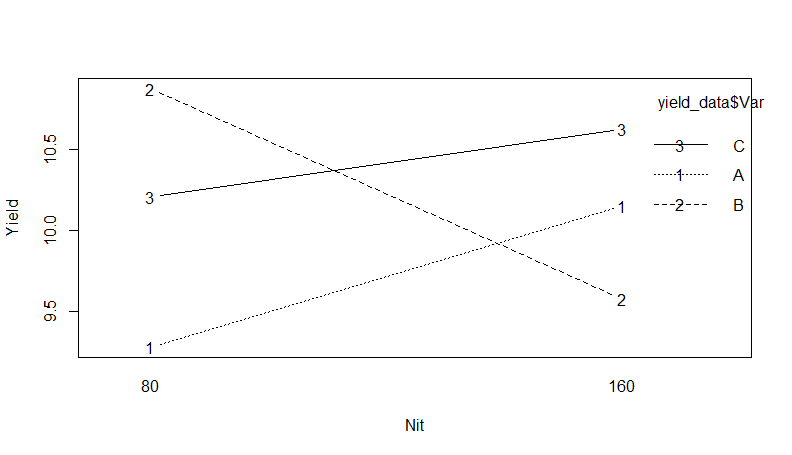
\includegraphics[width=0.6\textwidth]{cellMeanPlot.png}
\caption{\label{fig:frog2}}
\end{wrapfigure}
\end{center}

\textbf{{b)}}
The var and Nit are fixed effects and Rep is a random effect. Using the lme model, the interaction between VarB:Nit160 is significant.

\begin{lstlisting}[label=R Code,caption=Q5(b) R Code Output]
> yield_data.model <- lme(Yield ~ Var*Nit,
random = ~ 1|Rep,data = yield_data)
> summary(yield_data.model)
Linear mixed-effects model fit by REML
 Data: yield_data 
       AIC     BIC    logLik
  261.8217 279.339 -122.9109

Random effects:
 Formula: ~1 | Rep
         (Intercept) Residual
StdDev: 4.521311e-05  1.39152

Fixed effects: Yield ~ Var * Nit 
                Value Std.Error DF   t-value p-value
(Intercept)  9.285000 0.4016973 63 23.114419  0.0000
VarB         1.589167 0.5680858 63  2.797406  0.0068
VarC         0.925833 0.5680858 63  1.629742  0.1081
Nit160       0.870833 0.5680858 63  1.532926  0.1303
VarB:Nit160 -2.167500 0.8033946 63 -2.697927  0.0089
VarC:Nit160 -0.456667 0.8033946 63 -0.568421  0.5718
 Correlation: 
            (Intr) VarB   VarC   Nit160 VB:N16
VarB        -0.707                            
VarC        -0.707  0.500                     
Nit160      -0.707  0.500  0.500              
VarB:Nit160  0.500 -0.707 -0.354 -0.707       
VarC:Nit160  0.500 -0.354 -0.707 -0.707  0.500

Standardized Within-Group Residuals:
        Min          Q1         Med          Q3         Max 
-2.77933420 -0.45932974  0.04311831  0.61668162  2.32299879 

Number of Observations: 72
Number of Groups: 4 
\end{lstlisting}

\textbf{{c)}}

Here we are taking Yr as fixed effect as well as Var and Nit to get an interaction between the Yr, Var and Nit.
The random effect is the subject which is Rep.
When we include Yr to the fixed effect none of the interaction are significant but they are correlated. 

\begin{lstlisting}[label=R Code,caption=Q5(c) R Code Output]
> yield_data.model <- lme(Yield ~ Var*Nit*Yr,
random = ~ 1|Rep,data = yield_data)
> summary(yield_data.model)
Linear mixed-effects model fit by REML
 Data: yield_data 
       AIC      BIC    logLik
  246.5138 275.8346 -109.2569

Random effects:
 Formula: ~1 | Rep
         (Intercept) Residual
StdDev: 4.491289e-05 1.189809

Fixed effects: Yield ~ Var * Nit * Yr 
                   Value Std.Error DF   t-value p-value
(Intercept)    10.425000  1.717341 57  6.070432  0.0000
VarB           -2.510833  2.428687 57 -1.033823  0.3056
VarC           -3.339167  2.428687 57 -1.374886  0.1745
Nit160          0.560833  2.428687 57  0.230920  0.8182
Yr             -0.285000  0.420661 57 -0.677505  0.5008
VarB:Nit160     6.517500  3.434682 57  1.897556  0.0628
VarC:Nit160    -3.011667  3.434682 57 -0.876840  0.3843
VarB:Yr         1.025000  0.594904 57  1.722966  0.0903
VarC:Yr         1.066250  0.594904 57  1.792305  0.0784
Nit160:Yr       0.077500  0.594904 57  0.130273  0.8968
VarB:Nit160:Yr -2.171250  0.841322 57 -2.580761  0.0125
VarC:Nit160:Yr  0.638750  0.841322 57  0.759222  0.4508
 Correlation: 
               (Intr) VarB   VarC   Nit160 Yr     VrB:N160 VrC:N160
               VrB:Yr VrC:Yr N160:Y
VarB           -0.707                                                                   
VarC           -0.707  0.500                                                            
Nit160         -0.707  0.500  0.500                                                     
Yr             -0.980  0.693  0.693  0.693                                              
VarB:Nit160     0.500 -0.707 -0.354 -0.707 -0.490                                       
VarC:Nit160     0.500 -0.354 -0.707 -0.707 -0.490  0.500                                
VarB:Yr         0.693 -0.980 -0.490 -0.490 -0.707  0.693    0.346                       
VarC:Yr         0.693 -0.490 -0.980 -0.490 -0.707  0.346    0.693    0.500              
Nit160:Yr       0.693 -0.490 -0.490 -0.980 -0.707  0.693    0.693    0.500  0.500       
VarB:Nit160:Yr -0.490  0.693  0.346  0.693  0.500 -0.980   -0.490   -0.707 -0.354 -0.707
VarC:Nit160:Yr -0.490  0.346  0.693  0.693  0.500 -0.490   -0.980   -0.354 -0.707 -0.707
               VB:N160:
VarB                   
VarC                   
Nit160                 
Yr                     
VarB:Nit160            
VarC:Nit160            
VarB:Yr                
VarC:Yr                
Nit160:Yr              
VarB:Nit160:Yr         
VarC:Nit160:Yr  0.500  

Standardized Within-Group Residuals:
        Min          Q1         Med          Q3         Max 
-2.11273471 -0.65399172 -0.08317164  0.48064452  2.71682346 

Number of Observations: 72
Number of Groups: 4 
 
 
 
 
 
\end{lstlisting}
\end{document}